\documentclass[a4,12pt]{scrartcl}
\usepackage[margin=3cm]{geometry}
\usepackage[francais]{babel}
\usepackage[utf8]{inputenc}
\usepackage{amsmath}
\usepackage{graphicx}
\usepackage{subcaption}
\usepackage[colorinlistoftodos]{todonotes}
\usepackage{tabularx}
\usepackage{colortbl}
\usepackage{hyperref}
\usepackage{float}

\title{Réalité Virtuelle}
\subtitle{Étude documentaire}

\author{Corentin Smith}
\date{\today}

\begin{document}
\maketitle

\newpage
\tableofcontents

\newpage
\section{Introduction}

La réalité virtuelle semble être un sujet éternellement à la mode, et en même temps éternellement lointain. Les différents acteurs ne cessent depuis les années 80 de promettre des expériences extraordinaires pour les deux ou trois années à venir.

Qu'est-ce que la réalité virtuelle exactement ? Quels sont les différents systèmes qui la composent ? Et est-elle enfin à même de nous offrir les résultats promis depuis depuis les années 80 ?

C'est à ces questions que nous allons tenter de répondre dans cette étude documentaire.

\section{Définitions et histoire}

\subsection{Définition}

Commençons par définir précisément ce qu'est que la réalité virtuelle. Cette dénomination vient de l'anglais \emph{virtual reality}, traduit peut-être un peu trop littéralement (\emph{virtual} peut avoir le sens de \emph{quasiment}, \emph{presque}, ce qui correspondrait plus à un terme de \emph{quasi-réalité} que de réalité virtuelle). Il désigne donc une simulation de la présence physique dans un endroit réel ou imaginaire, faisant appel à différents sens. En pratique, les systèmes de réalité virtuelle se limitent principalement à la vue, l'ouïe et le toucher.

Nous nous concentrerons dans cette étude sur les systèmes portés par l'utilisateur (par opposition aux salles immersives, qui ne permettent pas de simuler les 3 dimensions en envoyant des images différentes aux deux yeux de l'utilisateur).


\subsection{Naissance}

Aussitôt qu'il a été possible d'afficher des images sur un écran d'ordinateur, les pionniers de l'informatique ont essayé d'utiliser ces capacités pour représenter un monde virtuel.

Le premier système pouvant s'apparenter à de la réalité virtuelle dans l'acception moderne du terme est sans doute le Sensorama de Morton Heilig \cite{Sensorama}. Sorti en 1962, il s'agit d'une station composée d'un écran, d'un diffuseur d'odeurs, de son stéréo, d'un siège vibrant, et d'un ventilateur destiné à simuler le vent dans les cheveux de l'utilisateur. Jusqu'à 4 stations peuvent être connectées afin d'avoir une expérience partagée.

\begin{figure}[H]
	\centering
	\begin{subfigure}{.4\textwidth}
	  \centering
	  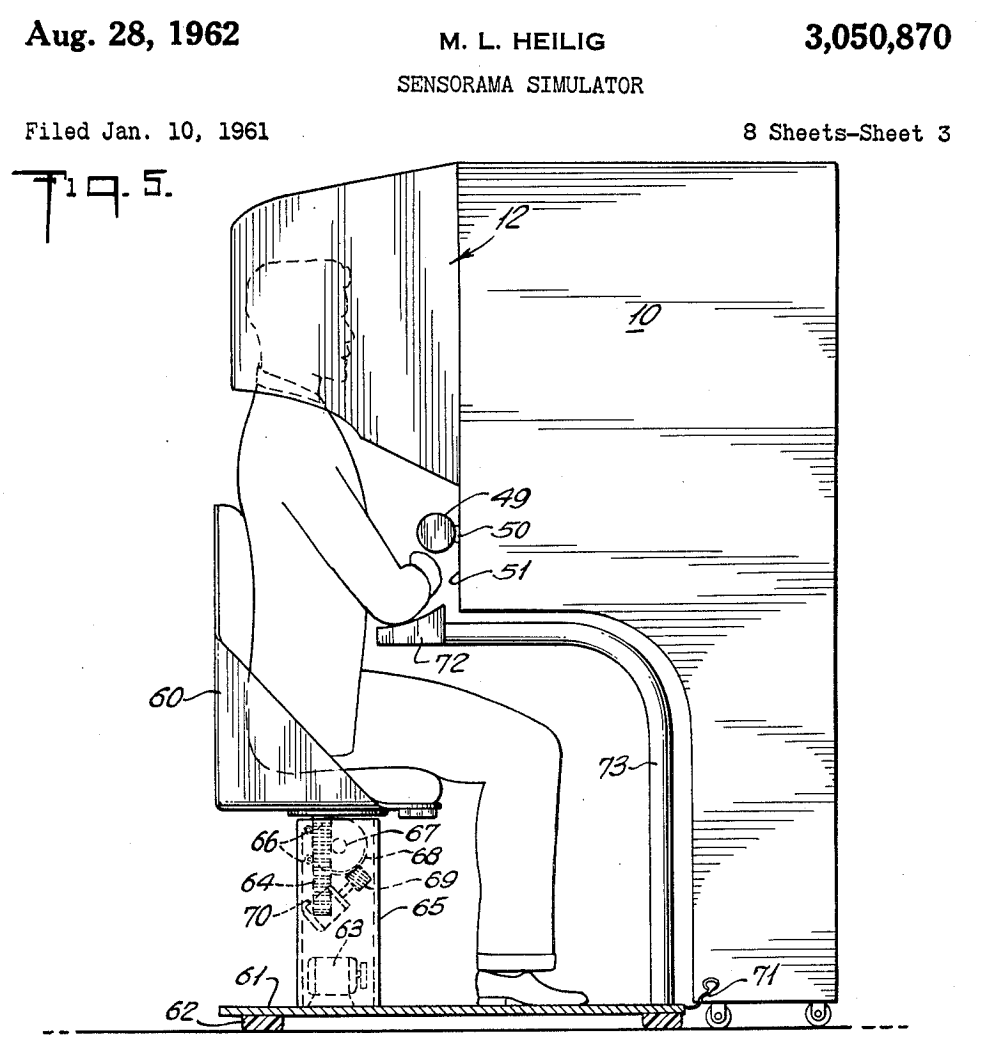
\includegraphics[width=\linewidth]{sensorama-patent}
	\end{subfigure}
	~
	\begin{subfigure}{.4\textwidth}
	  \centering
	  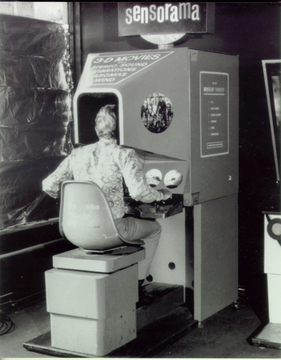
\includegraphics[width=0.8\linewidth]{sensorama}
	\end{subfigure}

 	\caption{Sensorama, Morton Heilig}
\end{figure}


\emph{L’épée de Damoclès}, nommée ainsi à cause de l’apparence extérieure du dispositif, est considérée comme le premier \emph{“visiocasque”}, ou \emph{head mounted display} (HMD) en anglais. Conçu par Ivan Sutherland et son équipe au MIT en 1968, il utilisait un système de suivi des déplacements externe, sous la forme d’un bras télescopique attaché au plafond. La visualisation était primitive, avec un affichage de graphismes 3D en fil-de-fer.

\begin{figure}[H]
	\centering
	\begin{subfigure}{.4\textwidth}
	  \centering
	  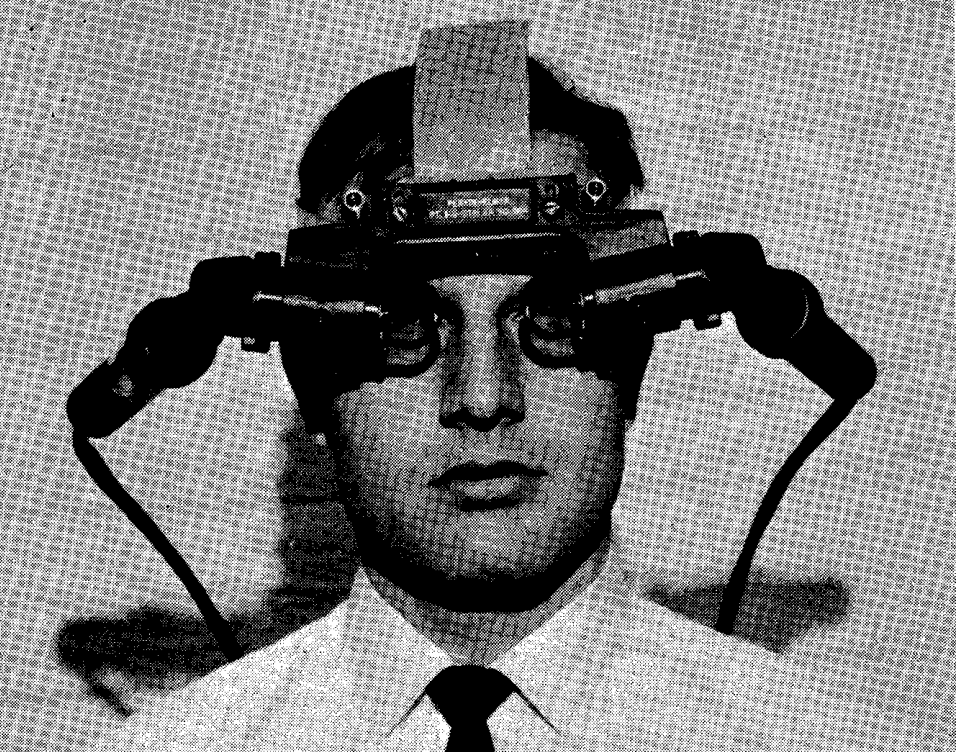
\includegraphics[width=\linewidth]{sutherland-1}
	\end{subfigure}
	~
	\begin{subfigure}{.4\textwidth}
	  \centering
	  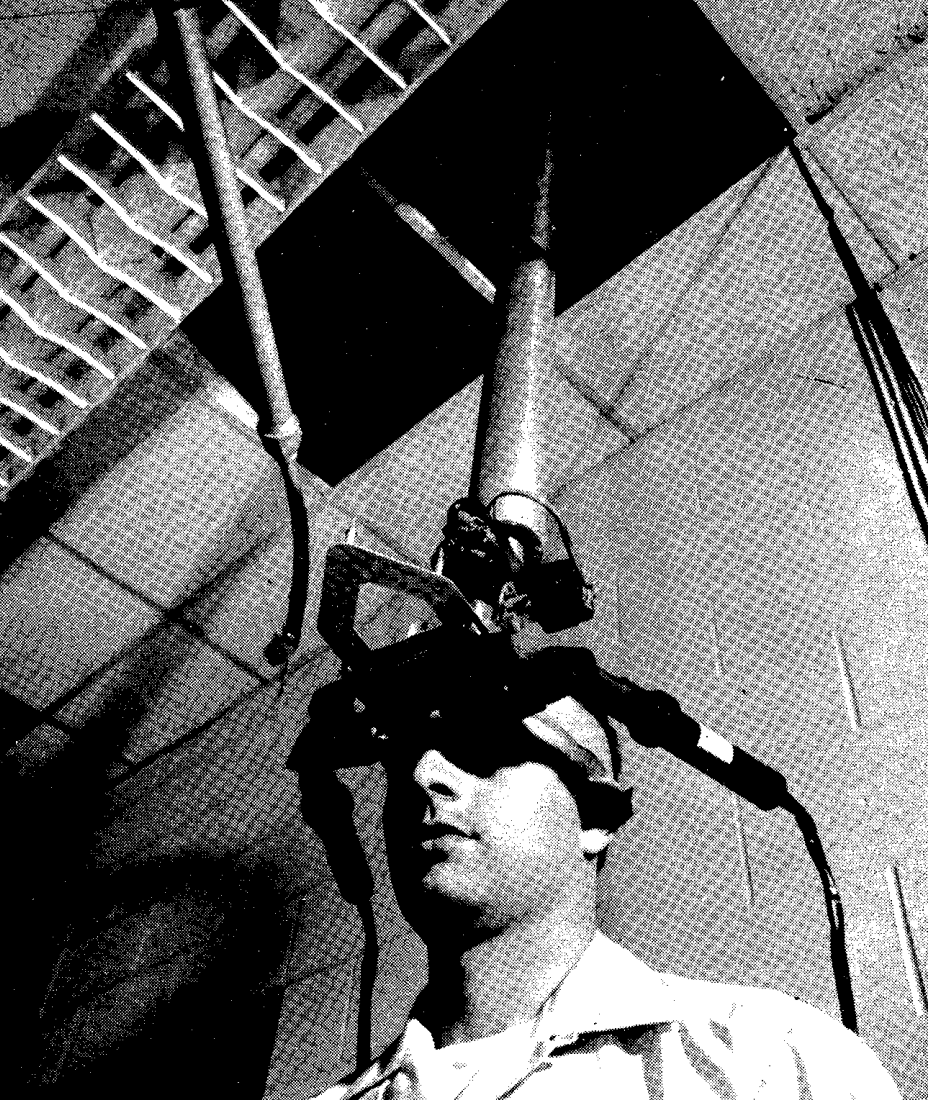
\includegraphics[width=0.8\linewidth]{sutherland-2}
	\end{subfigure}
 	\caption{\emph{L’épée de Damoclès}, Ivan Sutherland \cite{Sutherland68}}
\end{figure}

\subsection{Années 80}

Dans les années 80, la recherche s'intensifie, poussée par le développement de l’informatique personnelle et  par des investissement de la NASA et du département américain de la défense \cite{theverge14}.

\begin{figure}[H]
	\centering
	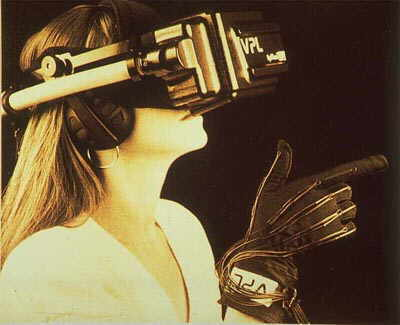
\includegraphics[width=0.6\linewidth]{vpl-hmd}
	\caption{Un système de VPL Research}
\end{figure}

Des start-ups commencent à émerger dans le domaine, notamment VPL Research, société de la Silicon Valley fondée par Jaron Lanier (qui est également connu pour avoir popularisé, et peut-être inventé le terme \emph{virtual reality}).

Les avancées de l'informatique permettent de commencer à afficher des mondes en trois dimensions rendus en temps réel avec des textures plus ou moins réalistes.

\subsection{Années 90}

Les années 90 sont en même temps l'âge d'or de la réalité virtuelle, et la mort de l'expérience grand public.

En 1991, \emph{Virtuality} lance le premier système de réalité virtuelle grand public. Il comportait des lunettes et des gants à exosquelette, ce qui en fait la première expérience immersive de réalité virtuelle. Vendu pour environ \$60 000 l'unité, il est destiné principalement au salles d'arcades.


La console Virtual Boy de Nintendo, sortie en 1995, est pour beaucoup le symbole de la réalité virtuelle, voire plus : le symbole de l'échec de la réalité virtuelle. Ce casque à vision binoculaire se posait sur une table, et était censé donner une sensation d'immersion très forte. Plusieurs problèmes cependant ont empêché le succès de l'appareil : la console n'affichait qu'une seule couleur, rouge, sur fond noir ; le système de bipied n'était pas du tout ergonomique ; et la plupart des personnes éprouvaient de fortes nausées en l'utilisant.

\begin{figure}[H]
	\centering
	\begin{subfigure}{.4\textwidth}
	  \centering
	  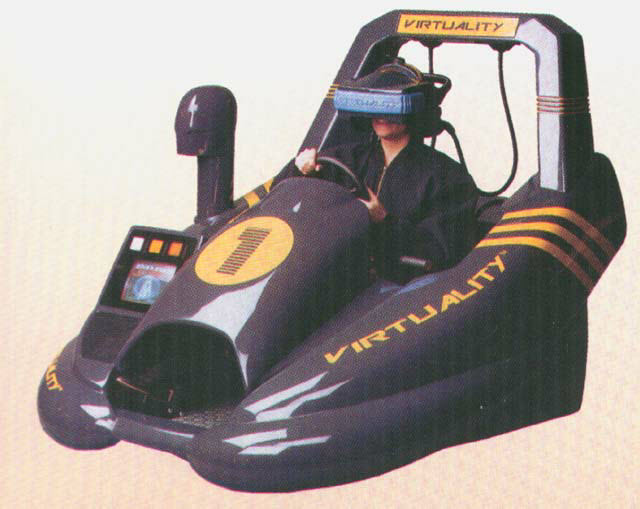
\includegraphics[width=\linewidth]{virtuality}
	  \caption{\emph{VR Pod} de Virtuality (1991)}
	\end{subfigure}
	~
	\begin{subfigure}{.4\textwidth}
	  \centering
	  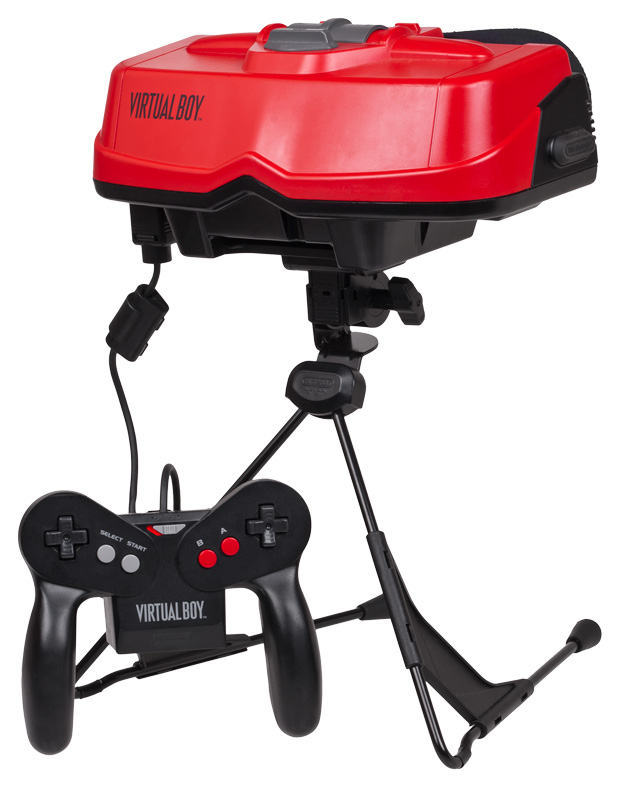
\includegraphics[width=0.8\linewidth]{virtualboy}
	  \caption{Nintendo Virtual Boy (1995)}
	\end{subfigure}
 	\caption{Systèmes de réalité virtuelle des années 90}
\end{figure}

Seulement une vingtaine de jeux ont été adaptés pour la console, et très peu vraiment immersifs (un bon nombre n'utilisaient pas l'effet 3D). Au final, ce fut donc un échec commercial cuisant, la production s'arrêtant moins d'un ans après le démarrage. 

De nombreuses autres sociétés tentent de percer dans le marché de la réalité virtuelle commerciale pendant la même période mais se heurtent de la même manière à des défis techniques insurmontables à l'époque et un marché assez peu réceptif. L'éclatement de la bulle internet dans les années 2000 finit d'achever l'expérience : on n'entendra quasiment plus parler de réalité virtuelle grand public avant le renouveau lancé par Oculus en 2012.

\subsection{Notion de présence}


Tous les systèmes de réalité virtuelle cherche à amener l'utilisateur dans un état de \emph{présence}. Il existe de nombreuses définitions de ce mot, que l'on peut trouver dans l'article de Schuemie et al. \cite{schuemie2001research}, mais qui se ramènent globalement à ce que le sujet n'arrive pas à distinguer \emph{à un niveau subconscient} que l'environnement dans lequel il se trouve n'est pas réel.

Michael Abrash \cite{Abrash14} cite l'exemple d'une scène dans laquelle l'utilisateur se trouve positionné en hauteur, comme sur un plongeoir surplombant une grande hauteur. Les textures formant les différents murs de l'environnement ne sont pas du tout réalistes, donc il n'y a aucun moyen de penser rationnellement que l'endroit (et donc le danger) est réel, et pourtant le fait de s'avancer au dessus du vide demande un effort conséquent (voire est impossible pour certaines personnes). Quelque part dans la chaîne de traitement de l'information, le cerveau indique qu'un danger est réellement présent, et la raison ne suffit pas toujours à le contredire !


\section{État de la technologie}

\subsection{Systèmes de vision}
\label{sysvis}

Les systèmes de vision pour la réalité virtuelle actuels se présentent à peu près tous sous la même forme : un ou deux écrans d’une dizaine de centimètres de diagonale sont placés sur une sorte de masque, couvrant les yeux de l’utilisateur. La position et/ou l’orientation de la tête sont mesurées par des capteurs internes ou externes, et l’utilisateur peut ainsi s’orienter dans le monde virtuel.\\

Michael Abrash liste dans sa conférence \cite{Abrash14} les différents paramètres les plus importants à prendre en compte dans les systèmes de vision pour arriver à une sensation de présence. Regardons ici les plus importants.

\subsubsection{Champ visuel}

Le champ visuel est défini comme l'ouverture angulaire dans laquelle l'utilisateur peut voir la scène virtuelle. Selon Abrash, la présence commence aux environs de 80 degrés d'ouverture et s'améliore significativement vers 110 degrés, ce qui correspond plus ou moins à la partie vision binoculaire du champ de vision humain. La plupart des appareils actuels ne dépassent pas 110 degrés de champ de vision.

\subsubsection{Résolution}

La résolution est un aspect évidemment très important d'une expérience de réalité virtuelle ; l'écran étant en général placé très proches des yeux de l'utilisateur, la résolution angulaire est assez faible en comparaison à un écran classique d'ordinateur ou de téléphone.

La résolution angulaire d'un \oe{}uil nu est de l'ordre d'une arcminute, ou $0,016$ degrés. Pour arriver à cette résolution angulaire avec un champ de vision de 110 degrés, il faudrait une résolution d'environ $6600 \times 6600$ (dans un format d'environ 4cm $\times$ 4cm si on place l'écran à une distance de 3cm de l'\oe{}uil, ce qui donne une densité de 4200 pixels par pouce).

On est donc encore loin d'être à ces niveaux de densité puisque les écrans les plus fins actuels arrivent tout juste à 500 pixels par pouce ; ce qui correspond au dernier prototype d'Oculus Rift, annoncé cette année au CES, qui est supposé avoir un écran de 2560 $\times$ 1440.

\subsubsection{Faible persistence}

La persistence est la durée pendant laquelle un pixel de l'écran reste allumé. Ce n'est pas un paramètre très important pour la plupart des écrans, mais dans le cas de la réalité virtuelle l'écran est placé très près des yeux, ce qui augmente le mouvement relatif de ces derniers par rapport aux pixels.

\begin{figure}[H]
	\centering
	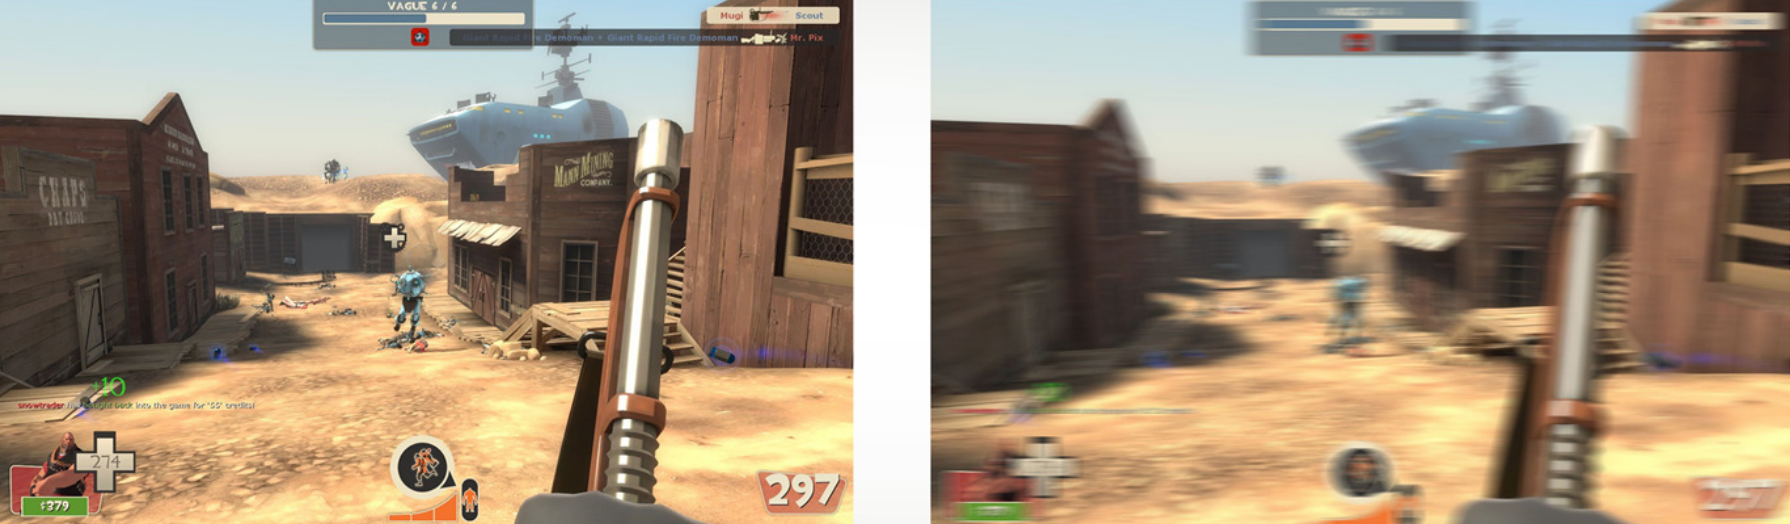
\includegraphics[width=\linewidth]{persistence}
	\caption{Simulation de l'effet de la persistence de l'image sur l'écran.}
\end{figure}

Une persistence de l'ordre de 3ms semble être suffisamment basse pour les systèmes actuels \cite{Abrash14}. Pour arriver à cette persistence, les écrans actuels utilisent des technologies OLED.

\subsubsection{Haut taux de rafraichissement}

Le fait de diminuer la persistence des pixels pose un problème visuel : l'image semble clignoter puisqu'elle est noire la plupart du temps. La persistence rétinienne ne suffit pas à compenser cet effet lorsque la fréquence de rafraichissement de l'image est trop faible.

En effet, à 60Hz, on a une image toutes les 16ms environ. Si chaque pixel ne reste allumé que 3ms, on a un “trou” de 13ms pour chaque image où l’écran n’affiche rien, ce qui est visible par l’utilisateur. Une fréquence de l’ordre de 95Hz semble être suffisante pour une expérience ne causant pas de nausées.


\subsubsection{Optique}

La conception du système optique d’un casque de réalité virtuelle est importante pour l’immersion. Un système idéal devrait permettre de régler simultanément : 
\begin{itemize}
	\item la distance focale
	\item la distance de visionnement
	\item la taille perçue de l’image
	\item la distortion
	\item les aberrations chromatiques
\end{itemize}

Cependant un système de cette nature devrait utiliser plusieurs lentilles en conjonction, et atteindrait des tailles et un poids qui ne sont pas en accord avec un dispositif pouvant tenir sur le visage de l’utilisateur (voir Figure~\ref{ideal-lens}).

\begin{figure}[H]
	\centering
	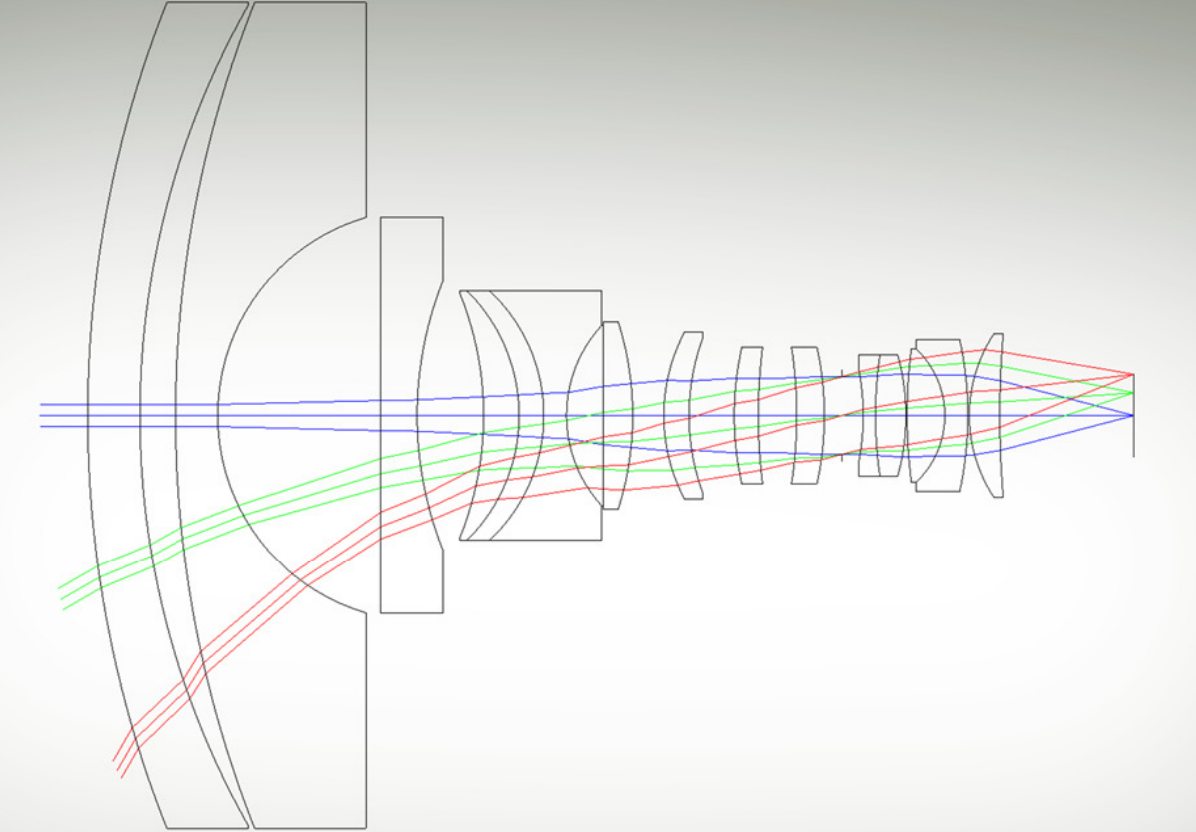
\includegraphics[width=0.6\linewidth]{lens}
	\caption{Système optique idéal (Valve) -- les plus grandes lentilles font plus de 30cm de diamètre}
	\label{ideal-lens}
\end{figure}

Un compromis est donc nécessaire dans la réalisation pratique, comme on peut le voir avec les lentilles de l’Oculus Rift, qui utilisent une forme carrée peu conventionnelle. Certains des défauts évoqués précédemment peuvent également être corrigés au niveau du logiciel, comme la distortion et l’aberration chromatique.

\begin{figure}[H]
	\centering
	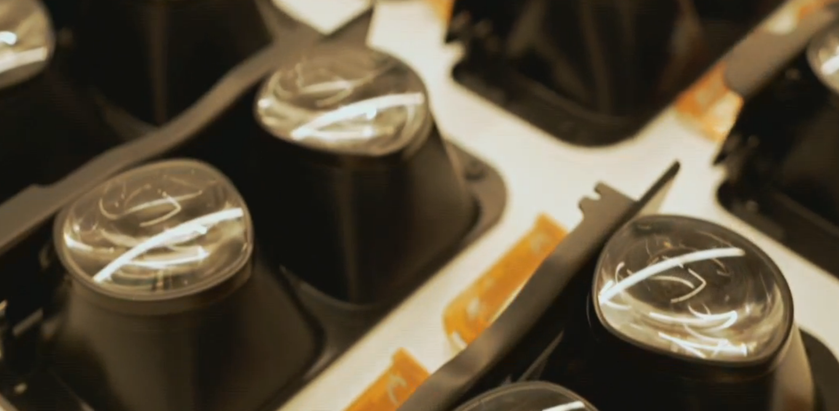
\includegraphics[width=0.7\linewidth]{crescent-bay-lens}
	\caption{Lentilles du dernier prototype de l’Oculus Rift}
\end{figure}

\subsubsection{Calibration optique}

Il ne suffit pas d’avoir de bonnes lentilles pour que les problèmes liés à l’optique soient réglés ; il faut également que le dispositif puisse s’adapter à l’utilisateur de manière très précise. Nous sommes extrêmement sensibles aux moindres erreurs de représentation du monde virtuel. Un exemple paramètre à régler individuellement est celui de la distance inter pupillaire, qui donne une information de taille aux objets vus dans la simulation.

\subsubsection{Tracking robuste}

Afin de retranscrire fidèlement les mouvements de l’utilisateur dans l’espace virtuel, une solution de tracking de la position et de l’orientation de la tête est nécessaire. Ce positionnement doit se faire de manière absolue, c’est-à-dire éviter la dérive. Une précision de l’ordre du millimètre dans les trois dimensions est requise.

\subsubsection{Temps de latence}

La perception du temps de latence est critique pour arriver à une sensation de présence.

Michael Abrash \cite{Abrash12} et John Carmack \cite{Carmack13} postulent qu’une latence \emph{“motion to photon”} de 20ms est la durée maximum pour ne pas être perceptible. Ceci pose problème car les technologies LCD ne sont pas conçues pour donner une faible latence.

Ceci oblige donc les constructeurs de matériel à recourir à travailler de très près avec leurs fournisseurs d'écrans pour concevoir des systèmes sur mesure ; ce qui donne un avantage considérable aux grands volumes dans la conception des systèmes, et donc aux constructeurs de matériel grand public.


\subsection{Systèmes audio binauraux}

Le champ de l’audio pour la réalité virtuelle est en train de prendre de l’ampleur, mais il n’a pas toujours été dans les priorités des constructeurs de matériel de réalité virtuelle.

\subsubsection{Principe de fonctionnement}

De la même manière que pour la vision binoculaire, la base du fonctionnement de l'audio binaurale réside dans la différence entre les signaux envoyés aux deux oreilles de l'utilisateur.

Le signal sonore voyage dans l'air à une vitesse constante, et arrive donc décalé aux deux oreilles. Cette subtile différence de temps suffit à localiser grossièrement la source du son.

Cependant, un son enregistré par des microphones classiques ne pourra pas être reproduit fidèlement par un casque, car la propagation des ondes sonores au voisinage des oreilles induit une réponse fréquentielle très particulière qui permet au cerveau de retrouver une information de localisation très précise.

\begin{figure}[!h]
	\centering
	\begin{subfigure}{.3\linewidth}
	  \centering
	  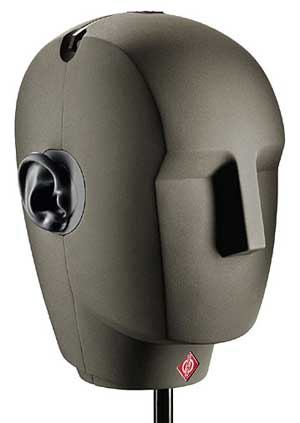
\includegraphics[width=0.8\linewidth]{ku-100}
	\end{subfigure}
	~
	\begin{subfigure}{.3\linewidth}
	  \centering
	  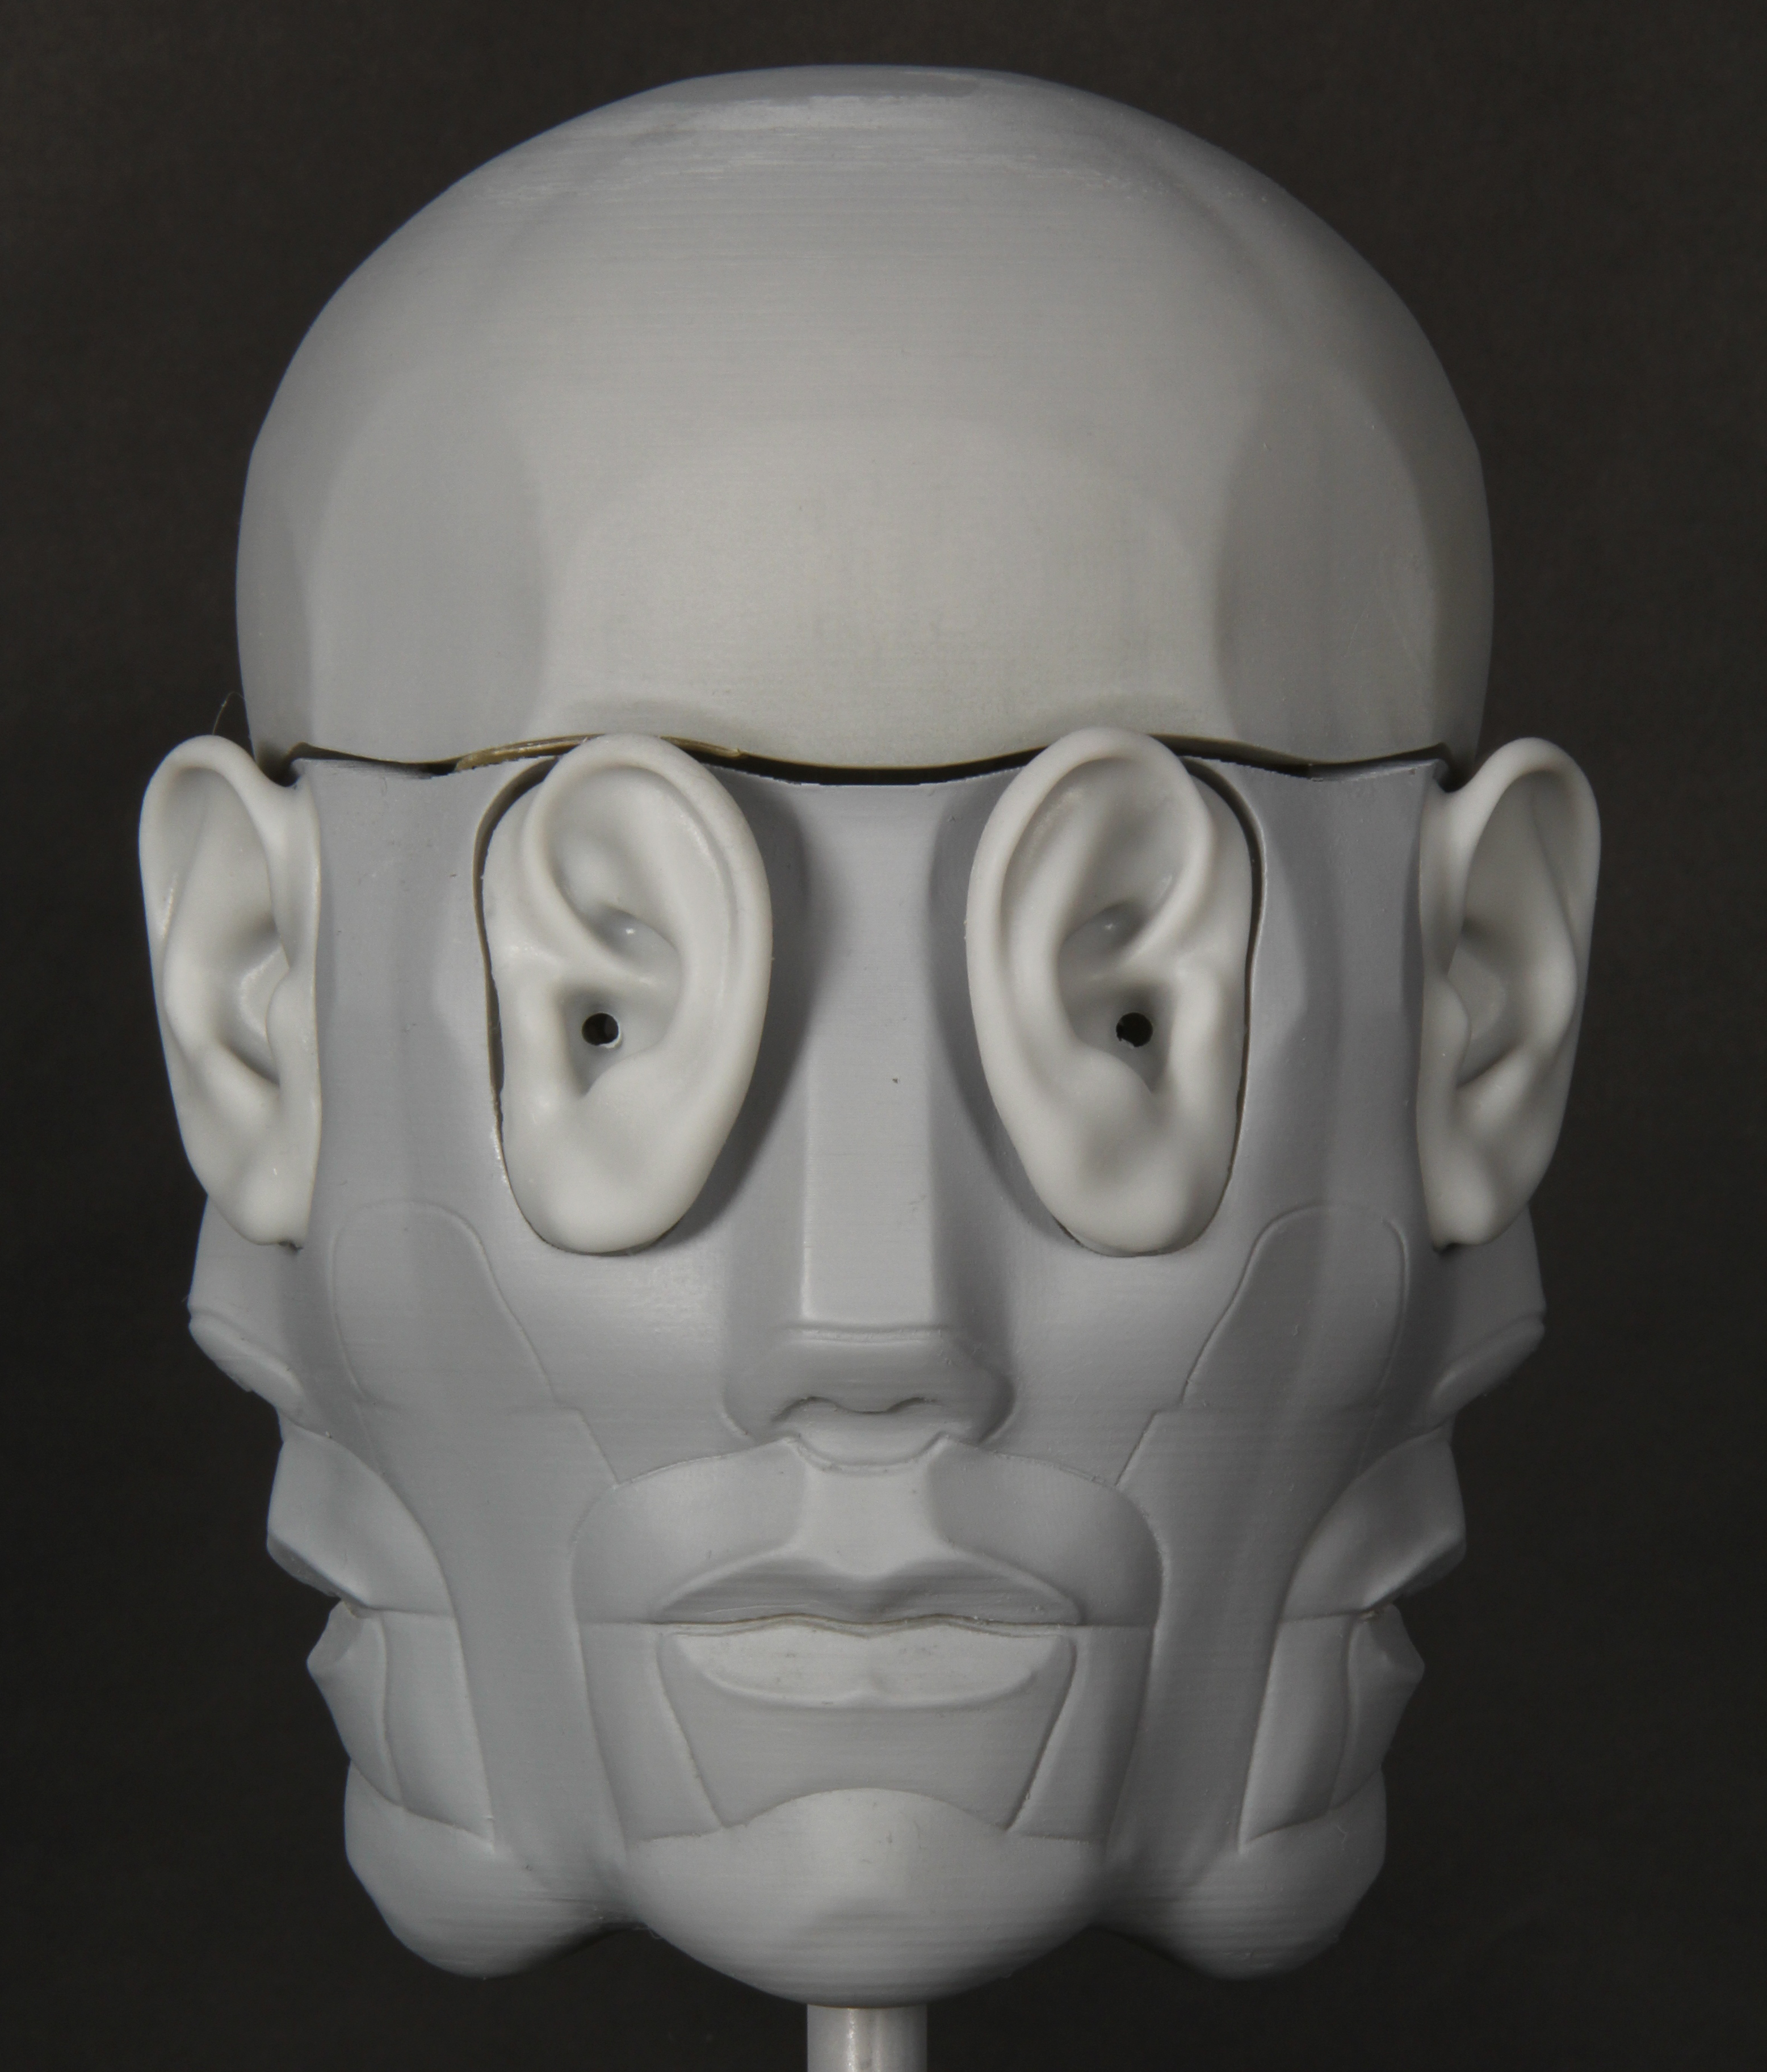
\includegraphics[width=\linewidth]{binaural-3d-microphone-head}
	\end{subfigure}
 	~
	\begin{subfigure}{.3\linewidth}
	  \centering
	  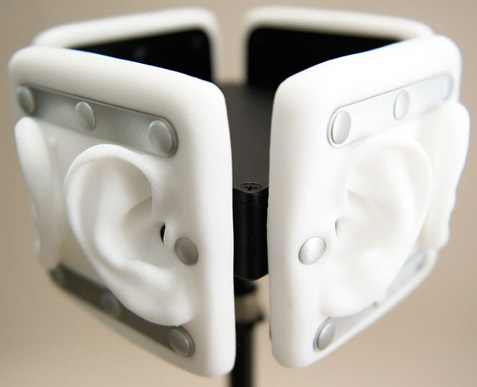
\includegraphics[width=\linewidth]{freespace-omni}
	\end{subfigure}
 	\caption{Différents micros pour enregistrement binaural}
 	\label{binaural}
\end{figure}

C'est pourquoi on a recours à des microphones binauraux, qui reproduisent la forme d'une oreille humaine, voire de toute une tête, afin d'arriver à la même fonction de transfert (on parle de \emph{Head-Related Transfer Function}). Écoutés au casque (c'est à dire sans perturbation de l'environnement), ces signaux enregistrés ont donc une réponse en fréquence très proche de la réalité.

\subsubsection{Problématiques}

L'enregistrement par ces techniques fonctionne extrêmement bien lorsque l'écoute est statique : il suffit de placer une tête d'enregistrement avec deux micros au niveau des oreilles, et la pratique est très convaincante.

Dès que l'auditeur peut évoluer dans son environnement (enregistrement vidéo à 360 degrés par exemple), tout se complique car on ne peut plus se contenter d'un seul enregistrement (si la personne fait un demi-tour par exemple, on inverserait les canaux de droite et de gauche).

Il faut donc avoir recours à des dispositifs d'enregistrement plus sophistiqués, comportant plusieurs micros (8 par exemple dans les dispositifs en fig. \ref{binaural}).

On a ensuite recours à des algorithmes de reconstruction tridimensionnelle, qui associent à chaque position une fonction de transfert équivalente.

\begin{figure}[!h]
	\centering
	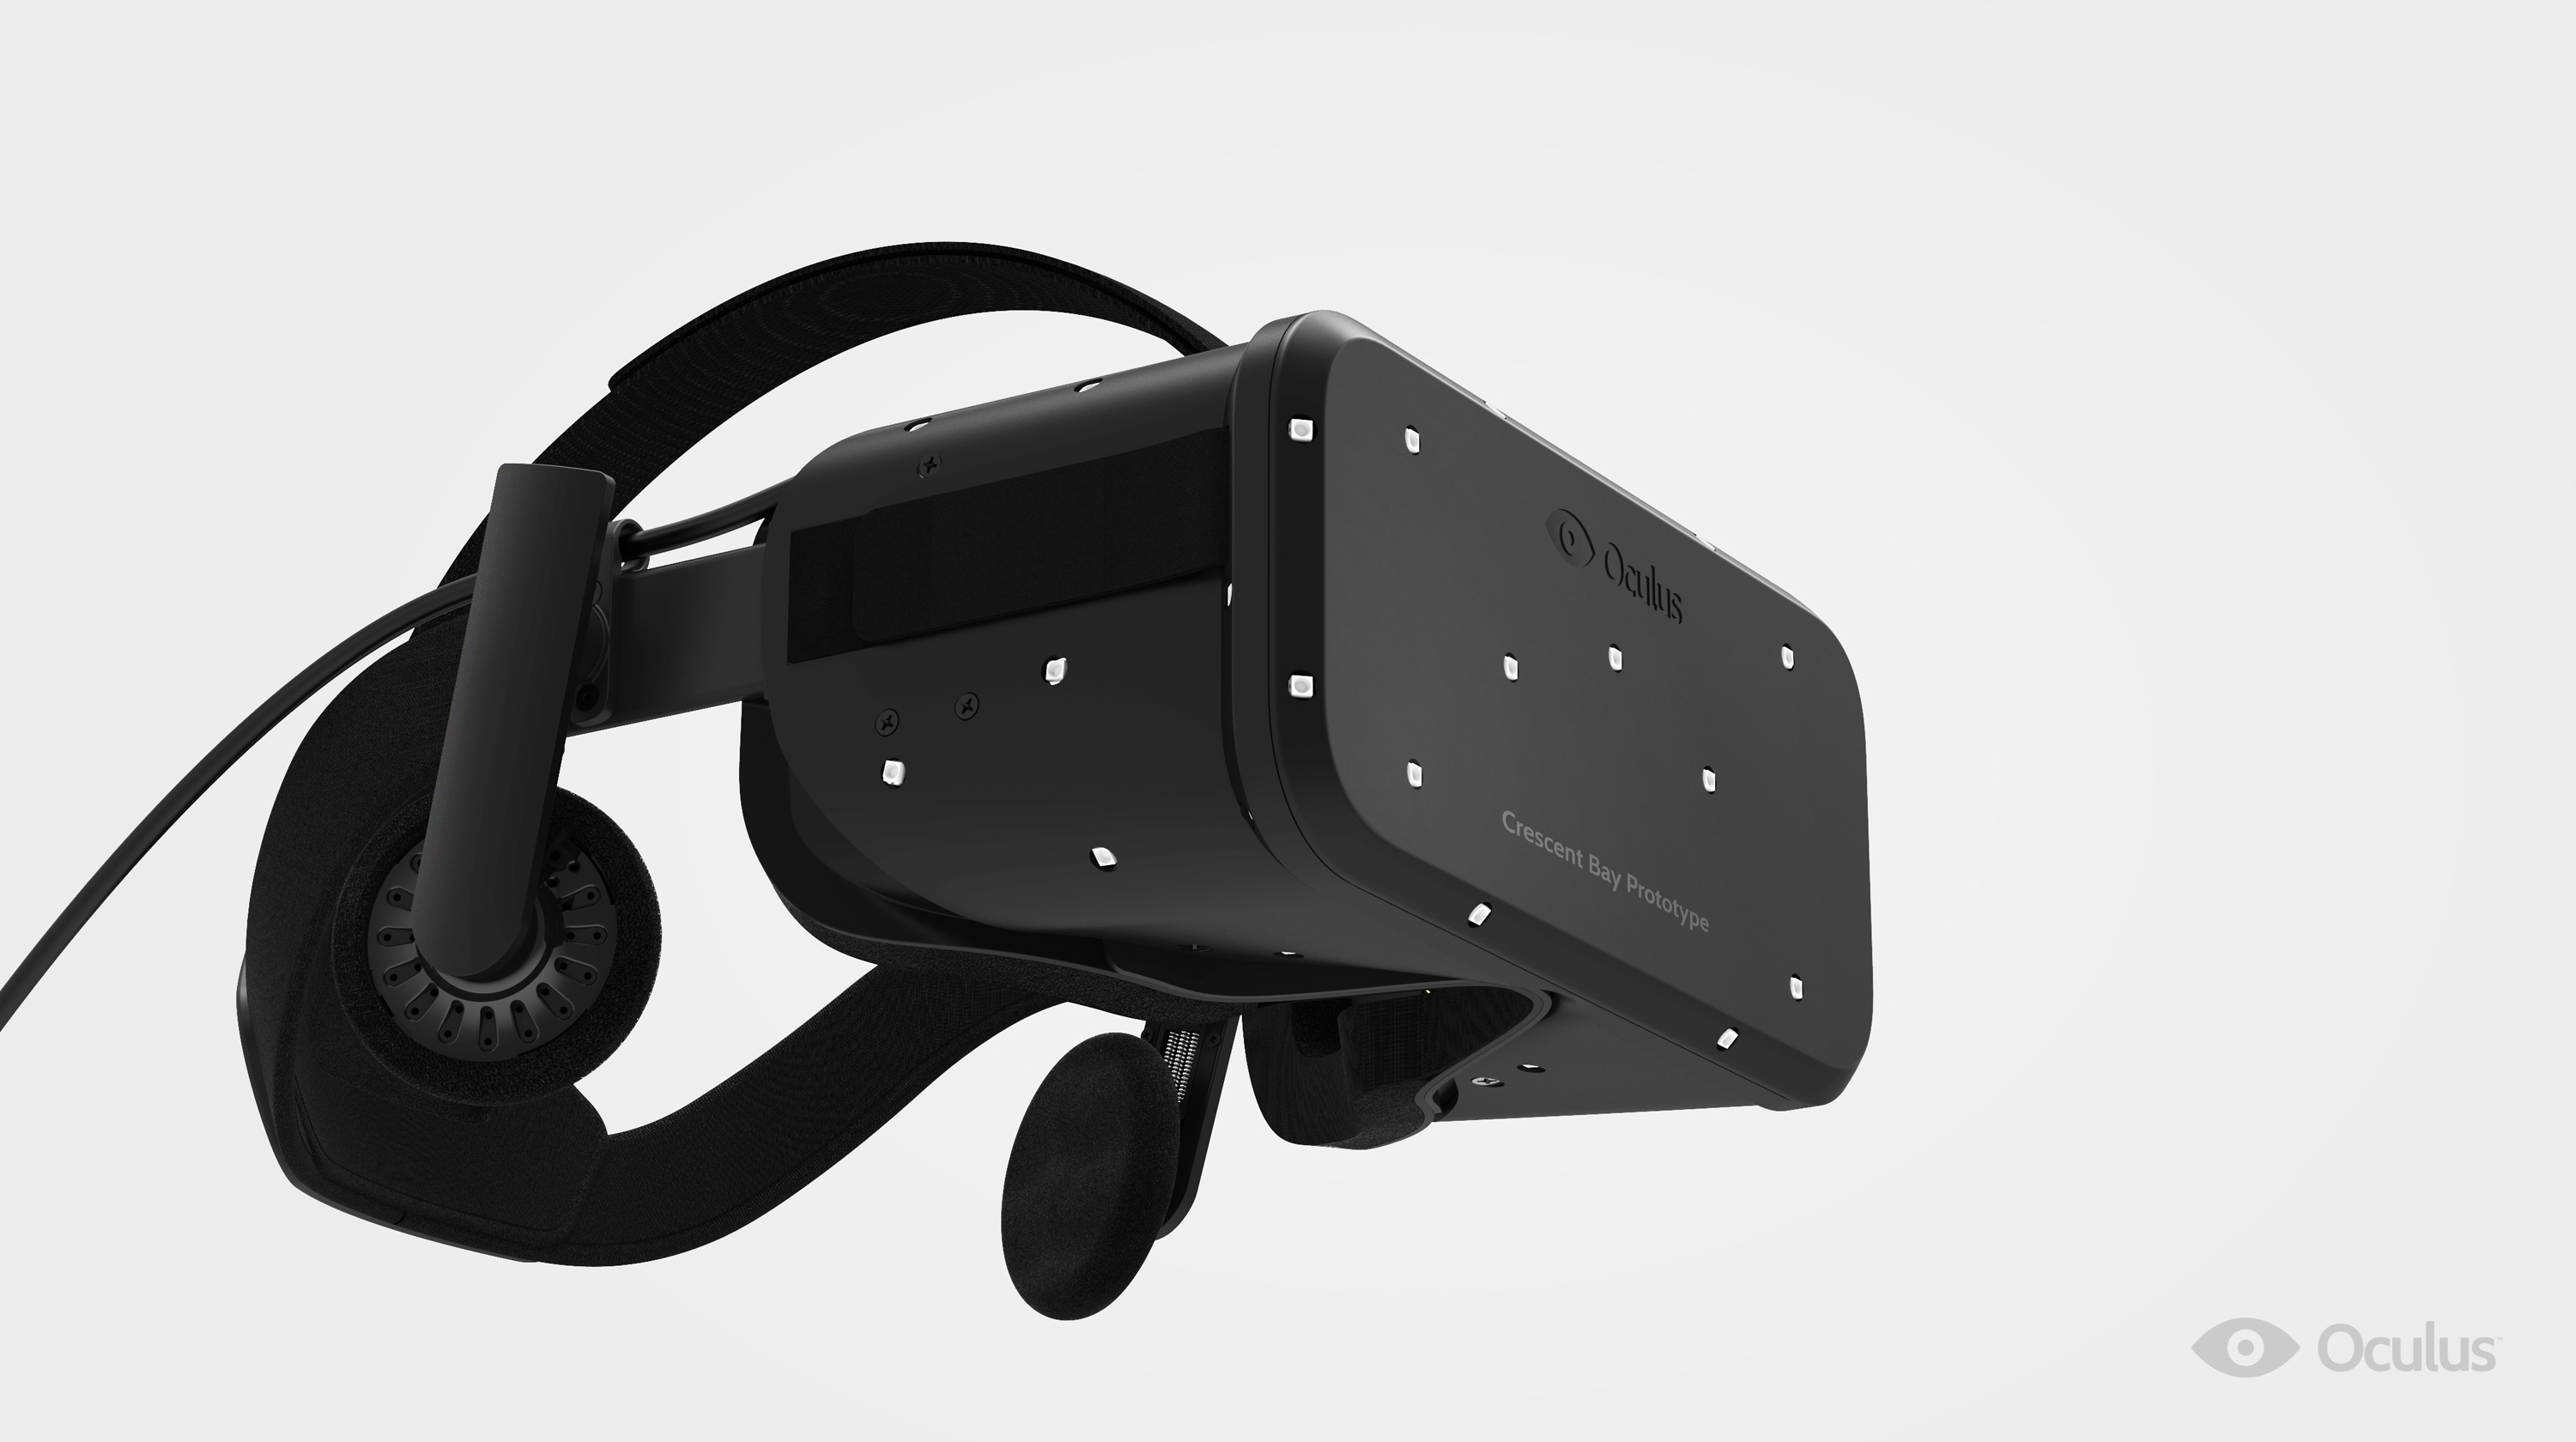
\includegraphics[width=0.6\linewidth]{crescent-bay}
	\caption{Le dernier prototype d'HMD Oculus comporte des écouteurs intégrés}
	\label{crescent-bay}
\end{figure}

Pour la plupart des expériences en réalité virtuelle, le paysage est généré de manière algorithmique et il n'y a donc pas d'enregistrement à proprement parler.

Les mêmes techniques sont cependant utilisées pour faire correspondre les sons émis à la position virtuelle de laquelle ils sont censés être émis. 

On observe une volonté de la part des fabricants de systèmes de réalité virtuelle d'inclure l'audio. La standardisation des écouteurs utilisés sera un facteur clé dans la réussite des effets de spatialisation puisque les éditeurs de contenu pourront alors compenser les fonctions de transfert intrinsèques au matériel et arriver à une qualité sonore suffisante pour bien distinguer les différents éléments.

\subsection{Systèmes maîtres/esclaves}

Les systèmes maître/esclaves désignent tous les équipements permettant de contrôler à distance un appareil (l'esclave) en manipulant une autre version de cette appareil localement (le maître). La version locale de l'appareil peut-être quasiment identique à l'esclave, ou bien être transformée pour une plus grande ergonomie. Par exemple, la manipulation d'un bras robotique de plusieurs mètres de long peut se faire avec une copie réduite du bras, facilement utilisable par un opérateur humain.


Dans le contexte de la réalité virtuelle, le système esclave est souvent un avatar de l'utilisateur dans le monde virtuel ; par exemple pour un gant haptique, l'utilisateur peut bouger une main virtuelle dans le monde qu'il observe grâce à son système de vision en utilisant sa main réelle dans le gant (le système maître).

\begin{figure}[H]
	\centering
	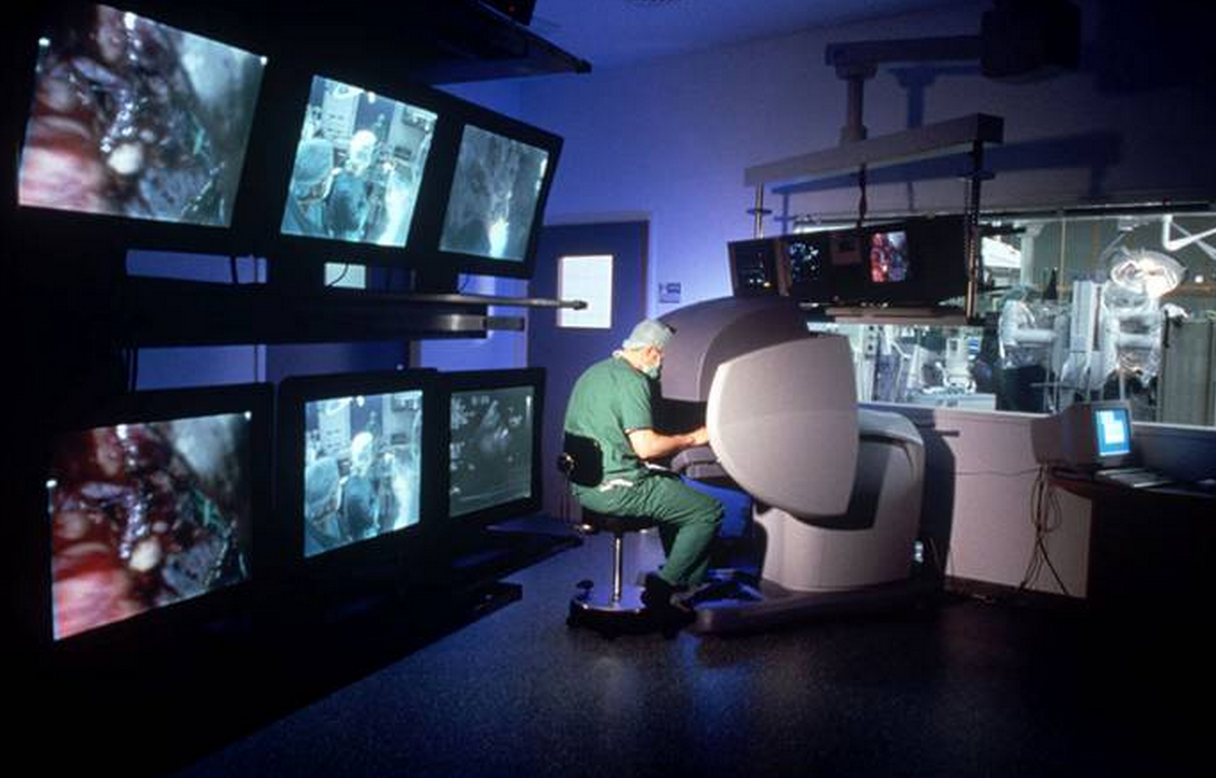
\includegraphics[width=0.6\linewidth]{operation}
	\caption{Téléopération}
	\label{operation}
\end{figure}

\subsubsection{Origine}

L'origine probable de ces systèmes est dans la manipulation des produits lourds et/ou dangereux dans l'industrie, ainsi que dans le spatial et dans le médical. C'est notamment dans le secteur du nucléaire que les systèmes les plus aboutis sont développés \cite{Garrec10}, avec en France la participation très active du CEA List, qui a réalisé au fil des années de nombreux systèmes allant de la simple tige téléopérée à l'orthèse de bras complète.  

Tout commence par un simple effet de levier : en bougeant une extrémité d'une tige, on peut avoir une action déportée sur un objet situé à l'autre bout. L'action est cependant inversée par symétrie centrale par rapport au point de levier, ce que l'on cherche généralement à éviter pour faciliter la manipulation.

Des systèmes complètement mécaniques à base de poulies sont donc apparus, permettant de déporter le mouvement de quelques mètres tout en gardant le même comportement des deux côtés. Il est toujours difficile d'avoir une grande distance entre les deux parties du système.

C'est pourquoi l'évolution naturelle des systèmes maîtres/esclaves tend vers la robotique, et s'applique naturellement à la réalité virtuelle. On coupe totalement les liens mécaniques entre le maître et l'esclave, remplacés par une liaison électrique. On peut alors choisir comme système esclave une représentation totalement virtuelle de l'objet à contrôler.


\begin{figure}[H]
	\centering
	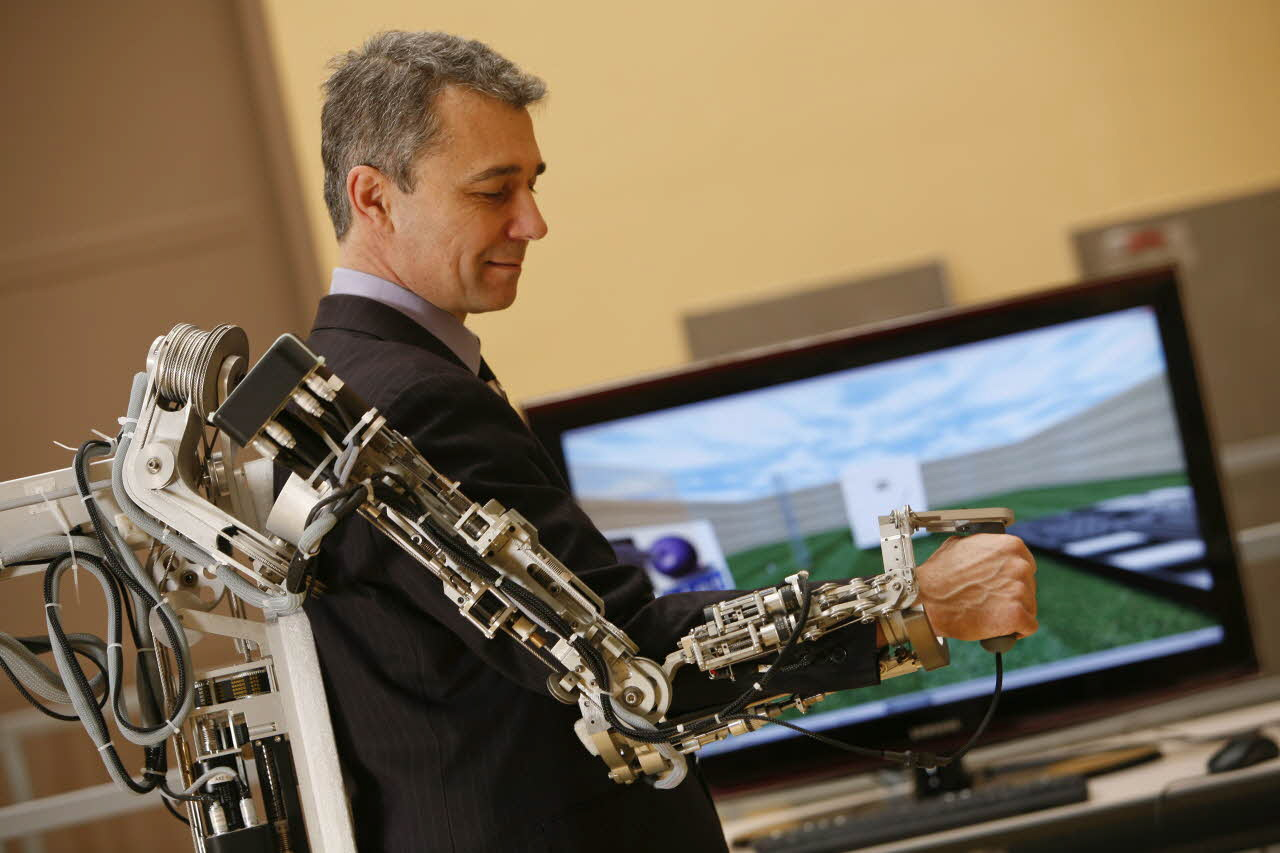
\includegraphics[width=0.6\linewidth]{garrec}
	\caption{Une orthèse du CEA List}
	\label{dexmo}
\end{figure}

\subsubsection{Paramètres clés}

Deux paramètres principaux viennent immédiatement à l'esprit : la fidélité de la reproduction du mouvement du maître par l'esclave, et la fidélité du retour donné par le maître lorsque l'esclave interagit avec son environnement.

Le temps de réponse doit être inférieur à une centaine de millisecondes pour être imperceptible pour la plupart des utilisateurs. Cette contrainte, bien qu'elle puisse sembler plus faible que sur les systèmes de vision, est en réalité très forte car les constantes de temps associées aux différents systèmes mécaniques mis en jeu sont beaucoup plus élevées.

Le développement de systèmes proprioceptifs nécessite donc souvent de la recherche et du développement sur de nouveaux actionneurs appropriés, très rapides, et suffisamment petits pour tenir sur le corps de l'utilisateur.

\subsubsection{Nouveaux entrants}

Les systèmes maîtres/esclaves se limitent pour l'instant à de très gros acteurs de la recherche et de l'industrie. Les séries sont très limitées, et les prix inaccessibles au grand public.

\begin{figure}[!h]
	\centering
	\begin{subfigure}{.4\linewidth}
		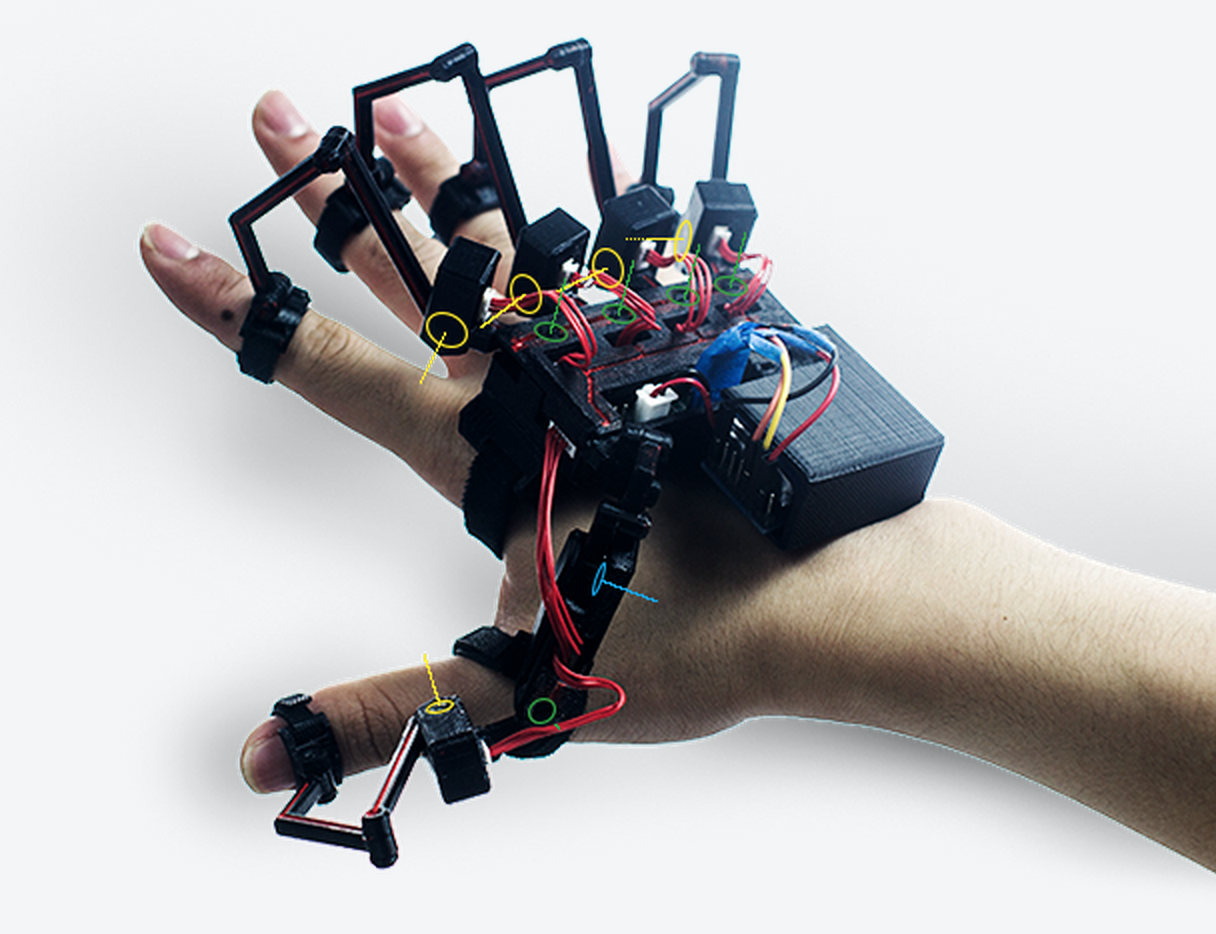
\includegraphics[width=0.8\linewidth]{dexmo}
		\caption{Dexmo F2, Dexta Robotics}
	\end{subfigure}
	~
	\begin{subfigure}{.4\linewidth}
		\centering
		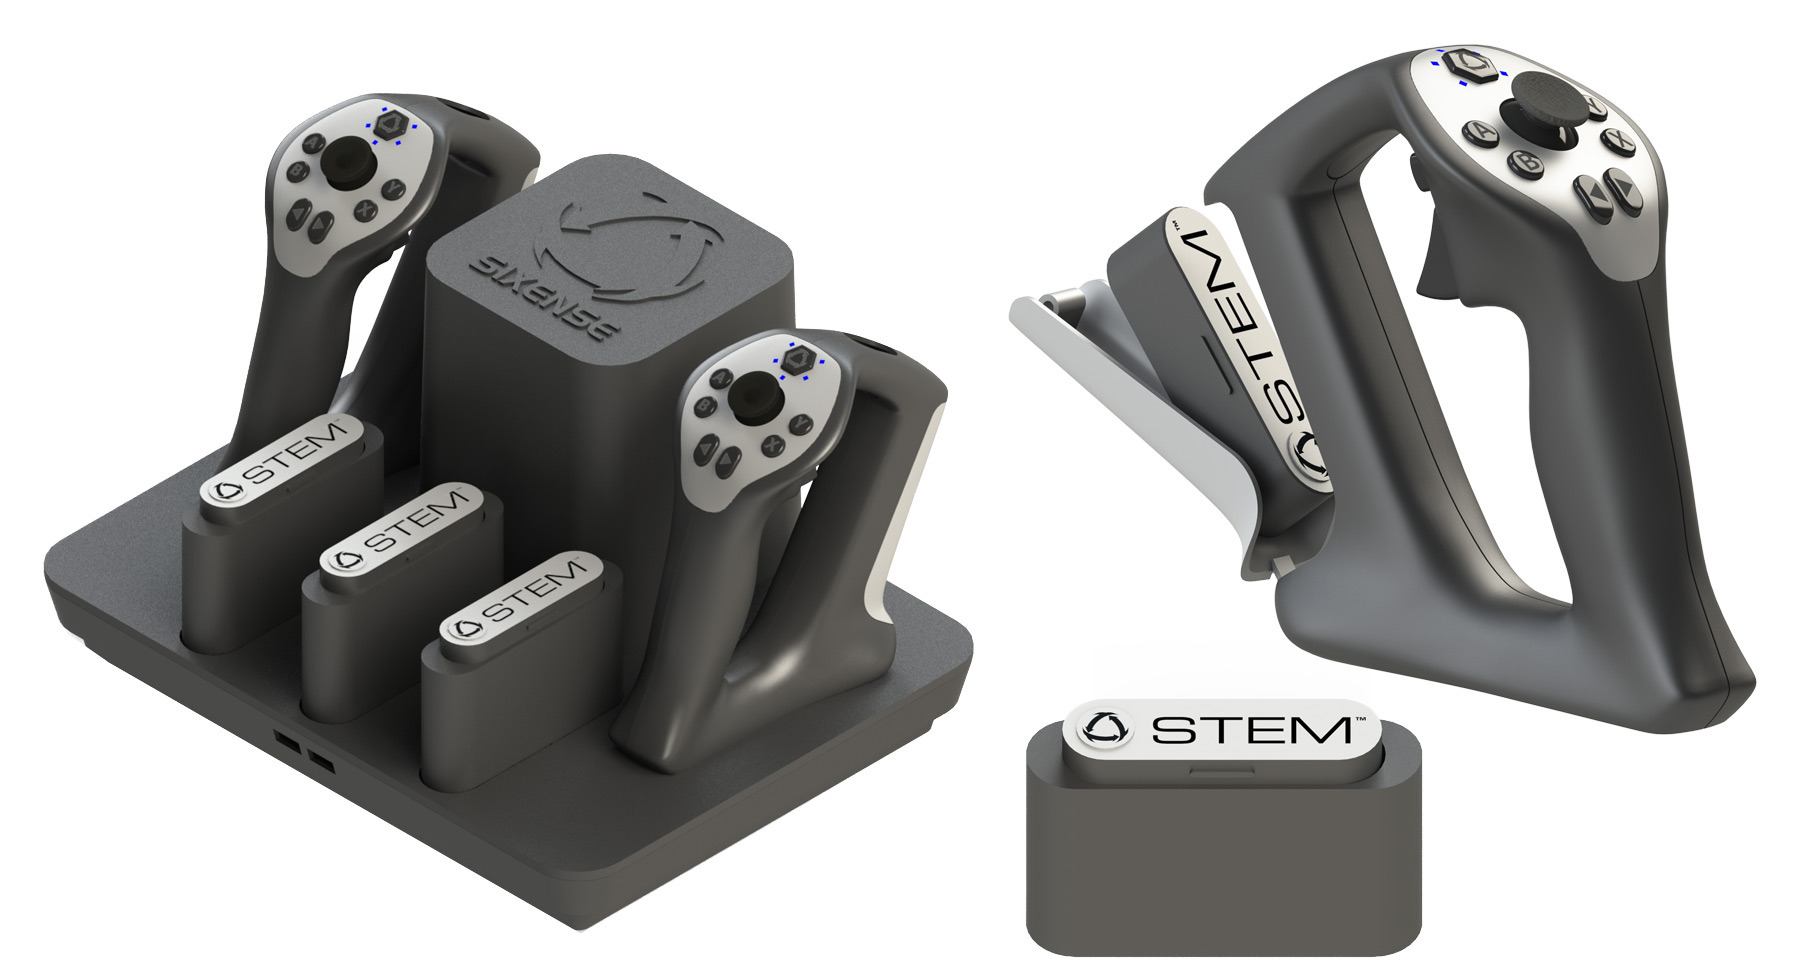
\includegraphics[width=\linewidth]{stem}
		\caption{Sixense STEM}
	\end{subfigure}
 	\caption{Nouveaux entrants}
 	\label{binaural}
\end{figure}


Avec l'arrivée d'Oculus et la promesse d'une révolution dans les prix des HMDs destinés au grand public, de nombreuses sociétés se sont créées ayant pour but de fournir des systèmes de commande pour la réalité virtuelle à un prix abordable.

Certaines, comme Dexta Robotics, tentent de proposer un exosquelette complet de main avec retour de force ; d'autres se focalisent sur la captation des mouvements sans retour de force. Cette deuxième solution est bien sur moins satisfaisante pour la réalité virtuelle puisqu'elle ne permet pas de ressentir son environnement par le toucher, et risque donc de casser l'immersion totalement. 

\begin{figure}[H]
	\centering
	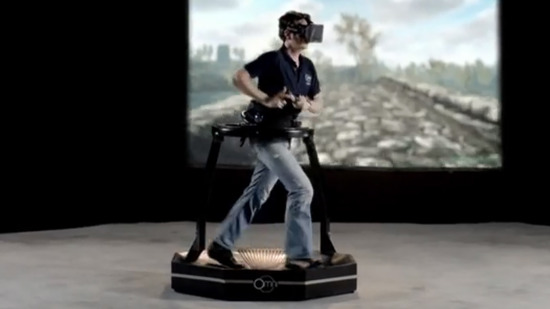
\includegraphics[width=0.6\linewidth]{omni}
	\caption{Virtuix Omni}
	\label{omni}
\end{figure}

Citons également à titre d'exemple l'Omni de Virtuix, qui propose un système visant à rendre les déplacements (marche et course) dans un environnement virtuel plus réalistes en fournissant un système de plateau glissant tenant l'utilisateur par la taille.

Tous ces systèmes sont pour l'instant à l'état de prototypes ou de premières petites séries. Il reste encore à convaincre qu'elles sont vraiment capables d'apporter un plus significatif dans l'immersion et la présence.

\section{Développements récents et futurs}

Après le grand flop des années 90, il a fallu attendre quasiment 20 ans pour que la réalité virtuelle revienne au goût du jour. Que s'est-il passé ?

La première réponse est que bien évidemment, la recherche ne s'est pas arrêtée pendant ces 20 ans. La réalité virtuelle est belle est bien utilisée tous les jours dans l'industrie, dans le domaine médical, dans la conception aéronautique et automobile, ou encore dans le nucléaire.

Cependant une personne est bien à l'origine du renouveau de l'engouement du grand public pour la réalité virtuelle.

\subsection{Oculus}

En 2012, Palmer Luckey est un jeune américain de 19 ans passionné de réalité virtuelle. Il collectionne les antiquité : des dizaines de casques et de lunettes des années 80-90 remplissent sa chambre et son atelier où il les démonte et les modifie dans le but de créer un meilleur système. Il tient quelques autres passionnés au courant de l'évolution de ses projets sur internet, et attire l'attention de John Carmack, un programmeur de haut profil, connu pour avoir créé plusieurs jeux à succès. Ils lancent une campagne de crowdfunding et récoltent plusieurs millions de dollars. Ils lancent un premier kit de développement, vendu à plus de 50 000 exemplaires, qui prouve le concept, et embauchent des grands noms de la R\&D en informatique graphique comme Michael Abrash.

En 2014, Facebook acquiert Oculus pour deux milliards de dollars.

Les derniers prototypes présentés par Oculus arrivent très proches des critères énoncés dans la partie \ref{sysvis}.

\subsection{Grand public enfin possible ?}

L'exemple d'Oculus fait bouger les choses dans les plus grandes sociétés : en 2014, Sony annonce qu'ils travaillent sur leur propre HMD, nommé \emph{Project Morpheus}. Microsoft se dirige plus vers la réalité augmentée en annonçant l'\emph{HoloLens}, des lunettes permettant de surimposer des objets virtuels sur le monde réel.

Dans le même temps, Google investit 500 millions de dollars dans une start-up appelée \emph{Magic Leap} qui promet une toute nouvelle technologie de réalité augmentée basée sur de la projection rétinienne.

Oculus a vendu depuis 2013 plus de 100 000 kits de développement.



Tout ceci semble très similaire à ce qui s'est passé dans les années 90, avec cependant une différence de taille : la technologie a évoluée de manière significative durant ces 20 dernières années, notamment grâce à l'industrie du smartphone qui a permis l'avènement d'écran haute résolution à bas prix, et l'évolution continue de la puissance de calcul des ordinateurs.

Il faudra pour aller plus loin que le contenu créé soit suffisamment attractif pour pousser les consommateurs à essayer de nouveaux appareils, et que le matériel soit disponible à un prix raisonnable. 2015 sera-t-elle l'année où la réalité virtuelle arrivera dans tout les foyers ?

\newpage
\bibliography{bibliography}
\bibliographystyle{plain}


\end{document}





